\clearpage
\section{Voltage determination}\label{sec:vol}
The voltage determination is a mot important and necessary part of this experiment. Before start it, we checked the gas system. we saw bubbles every few second at window on a test tube, so we were sure that the gas system was working.

\subsection{PMT operation voltage determination}
To determine the PMT operation voltage we have installed three counters. The leftmost counter shows the rate for the top panel, the middle counter shows the rate of bottom panel, and the rightmost counter shows the coincidence rate \cite{manual}. Then, we started to take count rate. We started to varying the voltage for bottom panel from \num{1700} V to \num{2300} V with in step of \num{50} V. At doing so, we were aware that voltage can't exceed of \num{2400} V for precaution. We took four measurements at every \num{10} second with every step of \num{50} V and calculated their averages to reduce the statistical errors. After measuring rate, we plotted a graph between average rate vs number of counts. In figure \ref{fig:PMTvoltageBot} we can see that initially the count rate increases exponentially with raising the voltage. Then it start to distribute linearly from 2000 V and follow completely linear distribution from \num{2100} V. Therefore, we took a working point at \num{2100}.\\

Afterward, we fixed the bottom voltage at \num{2100} V, then we vary the voltage for top panel as in before step in the same range. And, we measured the coincidence rate via rightmost counter. Unfortunately, the rightmost counter has broken, so last digit of count number is not clearly readable. It could lead some statistical error. By plotting a graph between measured voltage and coincidence rate we got a plateau curve \ref{fig:PMTvoltageTop}. From figure \ref{fig:PMTvoltageTop} it is clear that coincidence rate cannot follow any fixed distribution it is literally independent with applied voltage. Initially coincidence rate is increase exponentially then it reached a peak point so-called knee of the plateau curve. Then it start to raising again with increasing voltage and reached another peak. Therefore, we choose our working point \num{2150} V between these two peaks.

\begin{figure}[H]
\begin{center}
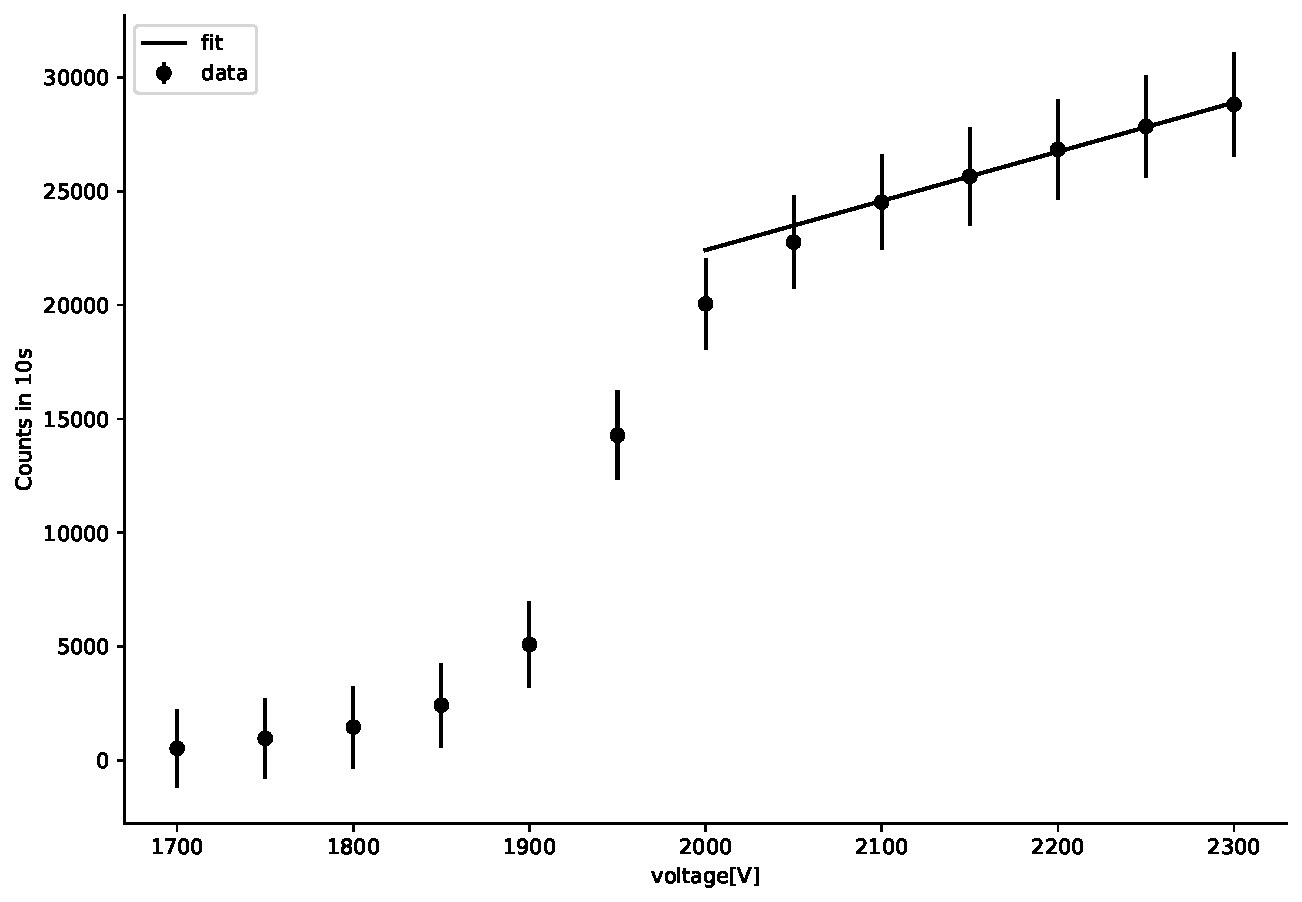
\includegraphics[width=0.6\linewidth]{bot.pdf}
	\end{center}
\caption{The number of counts for bottom panel with varying voltage.}
\label{fig:PMTvoltageBot}
	\end{figure}
	
	
\begin{figure}[H]
		\begin{center}
			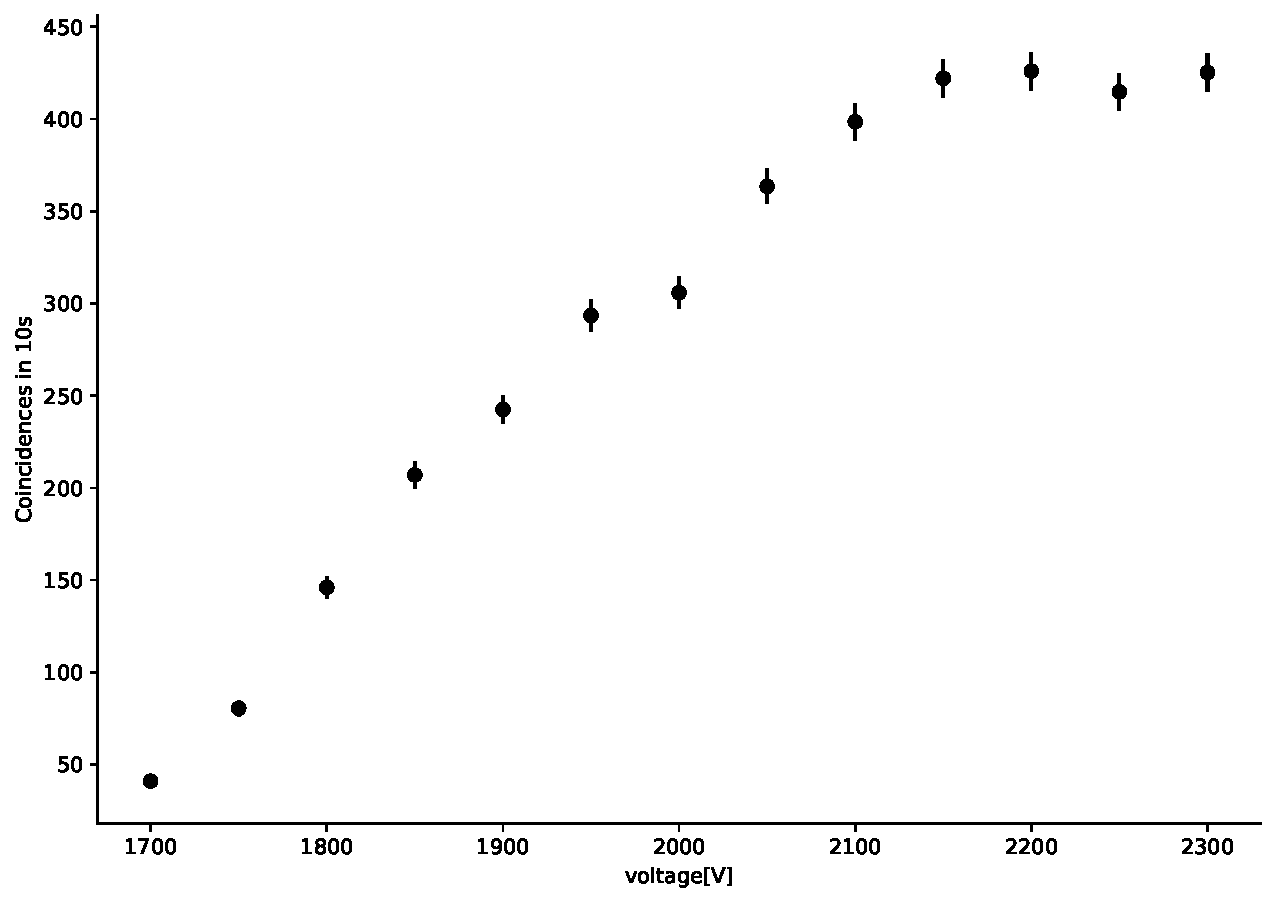
\includegraphics[width=0.6\linewidth]{top.pdf}
		\end{center}
	\caption{The number of counts for top panel with varying voltage.}%
	\label{fig:PMTvoltageTop}
\end{figure}	
	
\subsection{Determination of the front-end threshold voltage}	
We have to determine the the optimal voltage for the front-end chip. The voltage is adjusted using power supply \cite{manual}. The selected voltage established as threshold voltage due to FE chips and converted into detector pulses. To determine so, We processed as \verb|StyxM2C2 -N 2500 -o TS_14V.txt --all --no-clean -I /home/styx/data/etraxp114/te13085163152.hld| with data file \verb|StyxM2C2|. Here, we have taken \num{25000} events in every step of \num{0.4} V from \num{1.4} V to \num{2.6} V. Afterward, to do find good channels we made a \verb|root| file as \verb|StyxMonitor TS_14V_mon.txt|. 

Finally, we compared the measurements for one TDC number and one channel number using \verb|StyxThresholdScane| by a command \verb|StyxThresholdScane 1 5 TS_14V_mon.txt TS_26V_mon.txt TS_26V_mon.txt  TS_26V_mon.txt|.\\

To choose threshold voltage, first of all, we look at the rates files two of them are in fig \ref{fig:rate}, we can see that the hits in channel are decreases with increasing voltage. since, at low voltage there are some noises and at high voltage some of the signals are cut. Interestingly, hits in channel are fluctuate at different voltages in different channel; however, it is seen that at \num{20} V is fixed. therefore, we have had chosen that voltage as the threshold voltage. 

 
 
\begin{figure}[H]
	\centering
	\begin{subfigure}[t]{0.8\textwidth}
		\begin{center}
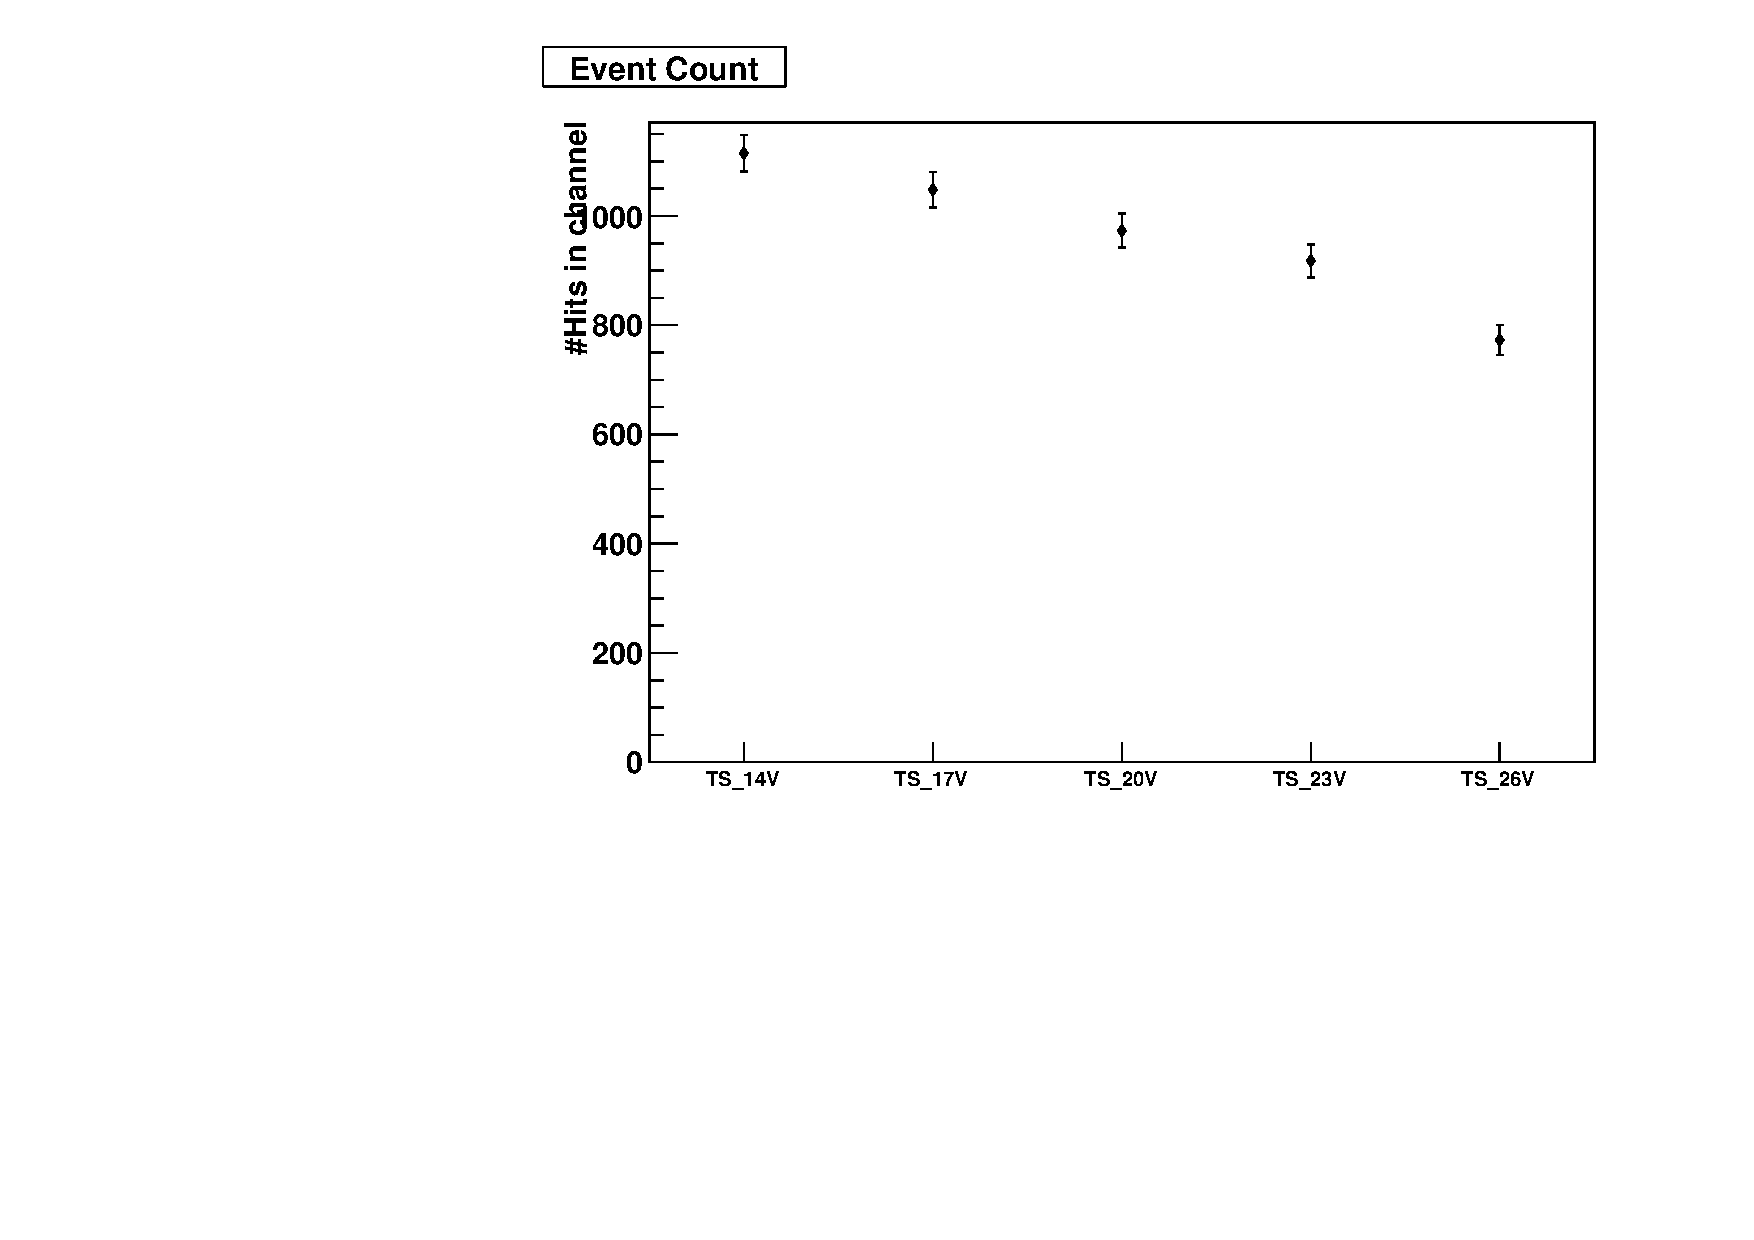
\includegraphics[width=0.8\linewidth]{StyxThresholdScan_1_2_Rate.pdf}
		\end{center}
		\caption{At TDC 1 channel 2.}
	\end{subfigure}
	
	\begin{subfigure}[t]{0.8\textwidth}
		\begin{center}
	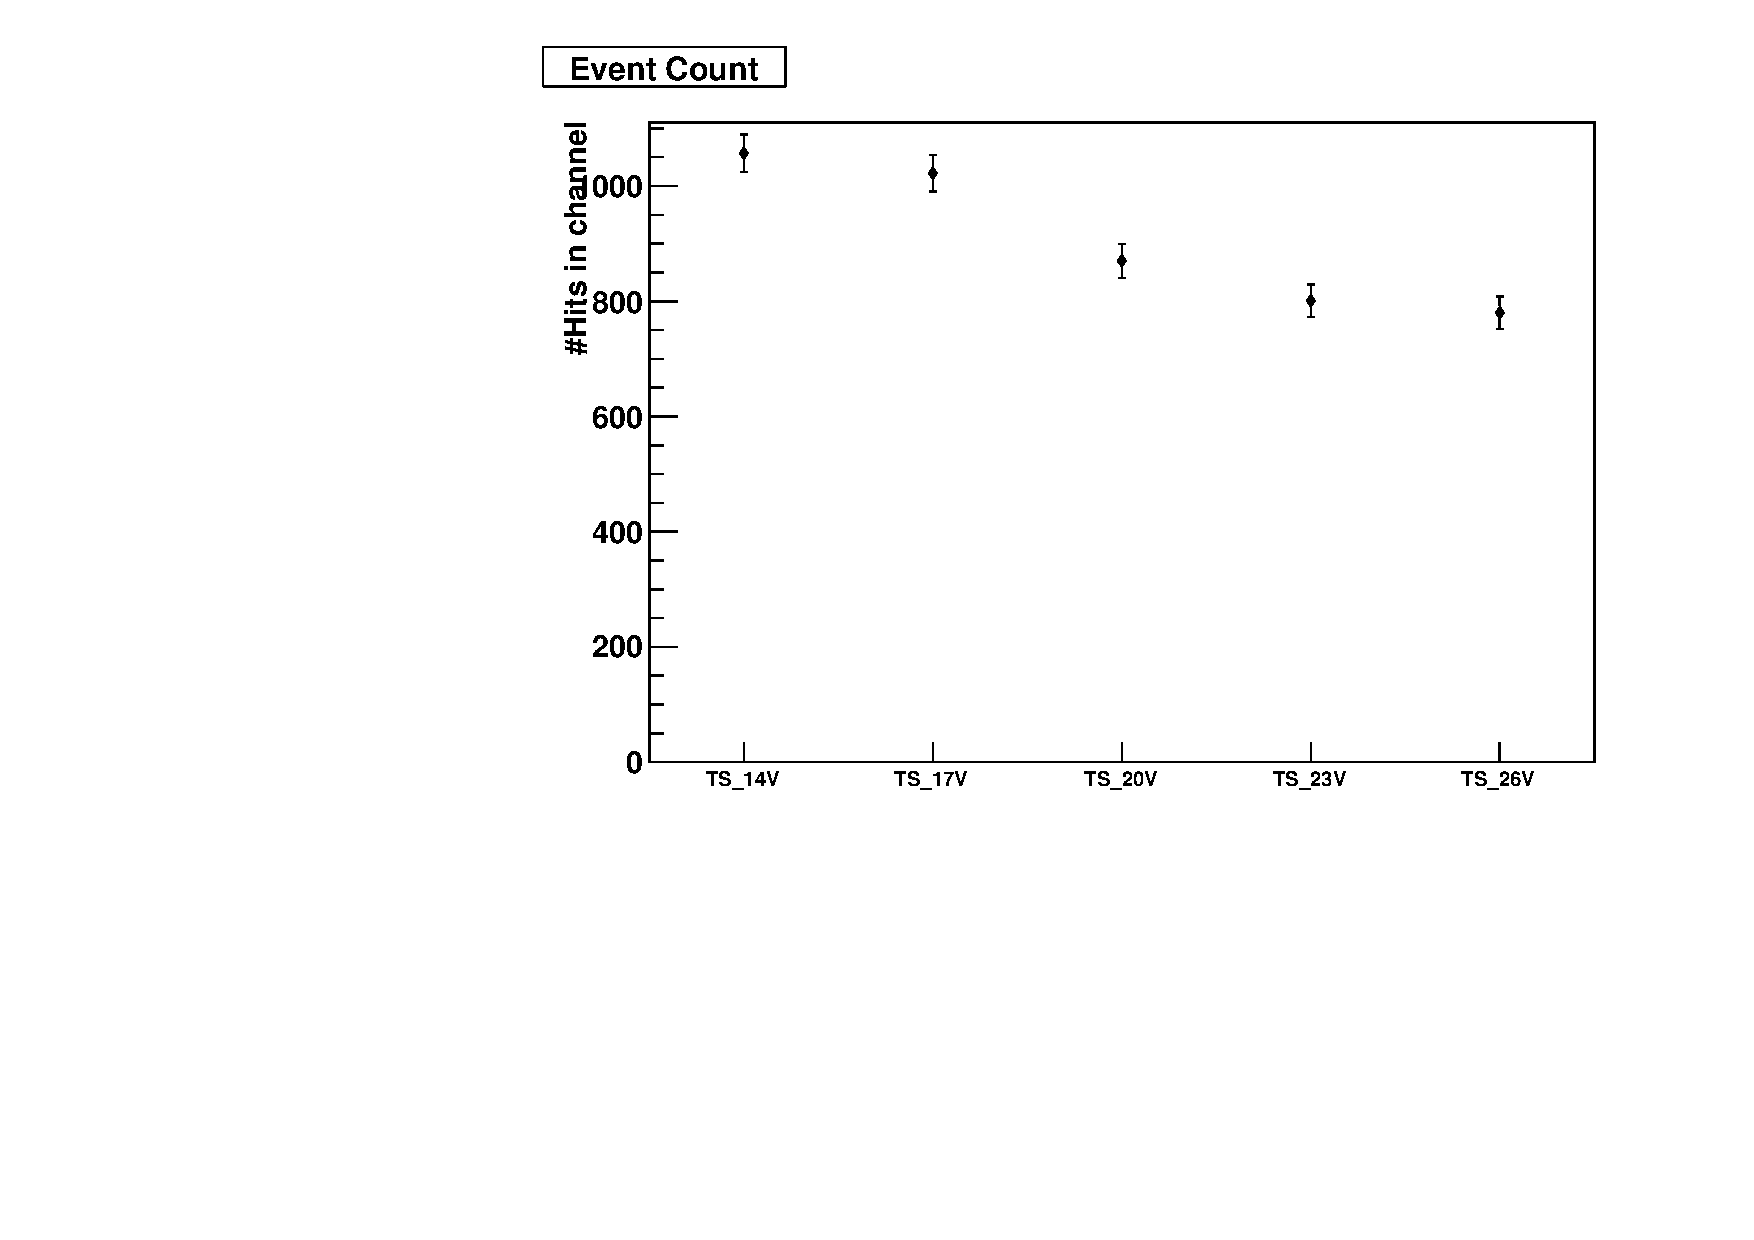
\includegraphics[width=0.8\linewidth]{StyxThresholdScan_1_5_Rate.pdf}
		\end{center}
		\caption{At TDC 1 channel 5.}
	\end{subfigure}
	\caption{The rate file of time vs hits in TDC 1 channel 2 at different voltages.}%
	\label{fig:rate}
\end{figure}

After that, we compared the overlay plots of different channels at different voltages. Two of them are in fig \ref{fig:Overlay}. We can see the relation between time-multiplexed of six straws with hits. The six output channels are condensed into one at the cost of having \num{1200} ns read out window per event \cite{manual}. From figure \ref{fig:Overlay},in several peaks for different straws, we can see that the noise level is too high at low voltage and heights of these peaks are quite different. The, also, peaks at \num{2.0} V seems quite same for all channels, but not at all other voltages. We want to find the lowest voltage so that the peaks seem to be of the same heights we can see it at \num{20} V. Therefore we choose the threshold voltage is \num{2.0} V.

\begin{figure}[H]
	\centering
\begin{subfigure}{0.8\textwidth}
 \begin{center}
 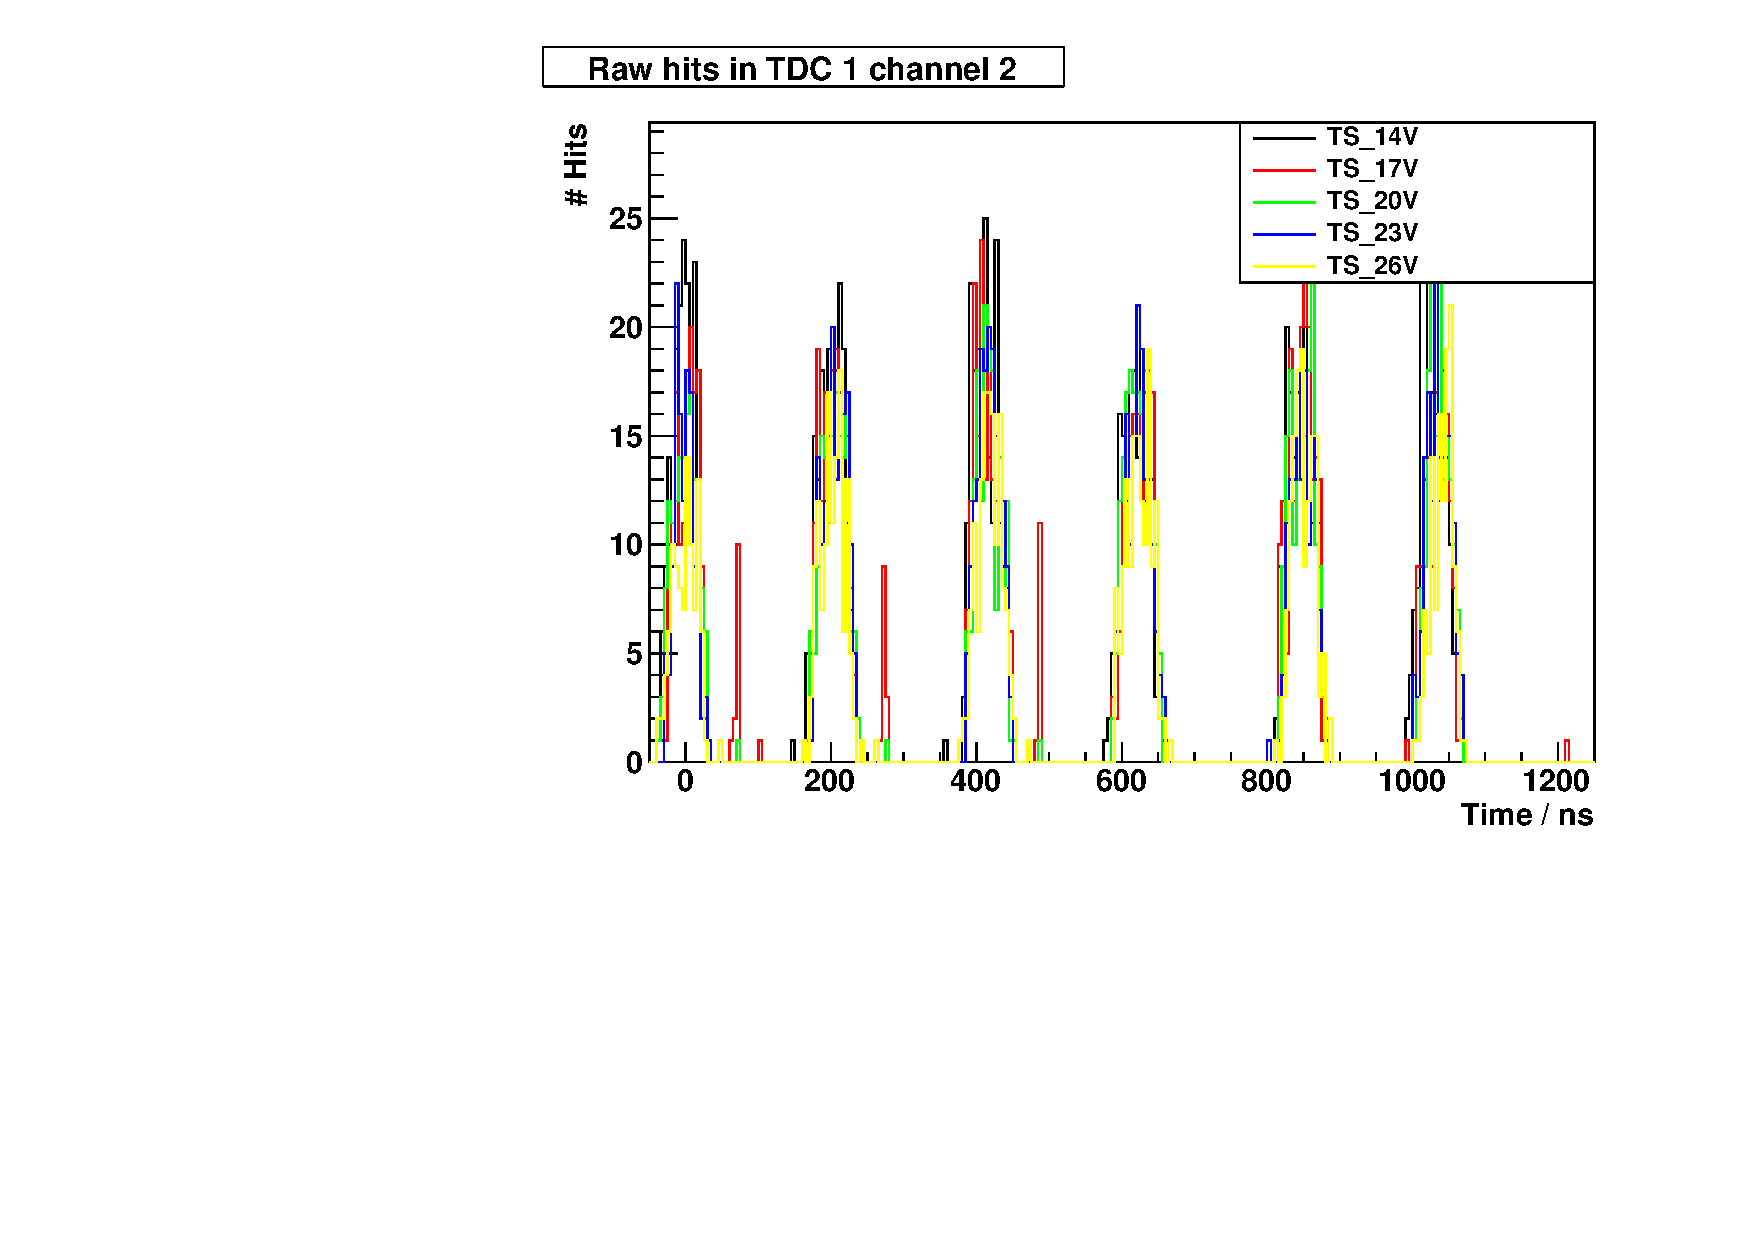
\includegraphics[width=0.8\linewidth]{StyxThresholdScan_1_2_Overlay.pdf}
 \end{center}
 	\caption{In TDC 1 channel 2 at different voltages.}
 \end{subfigure}
 
 \begin{subfigure}{0.8\textwidth}
 	\begin{center}
 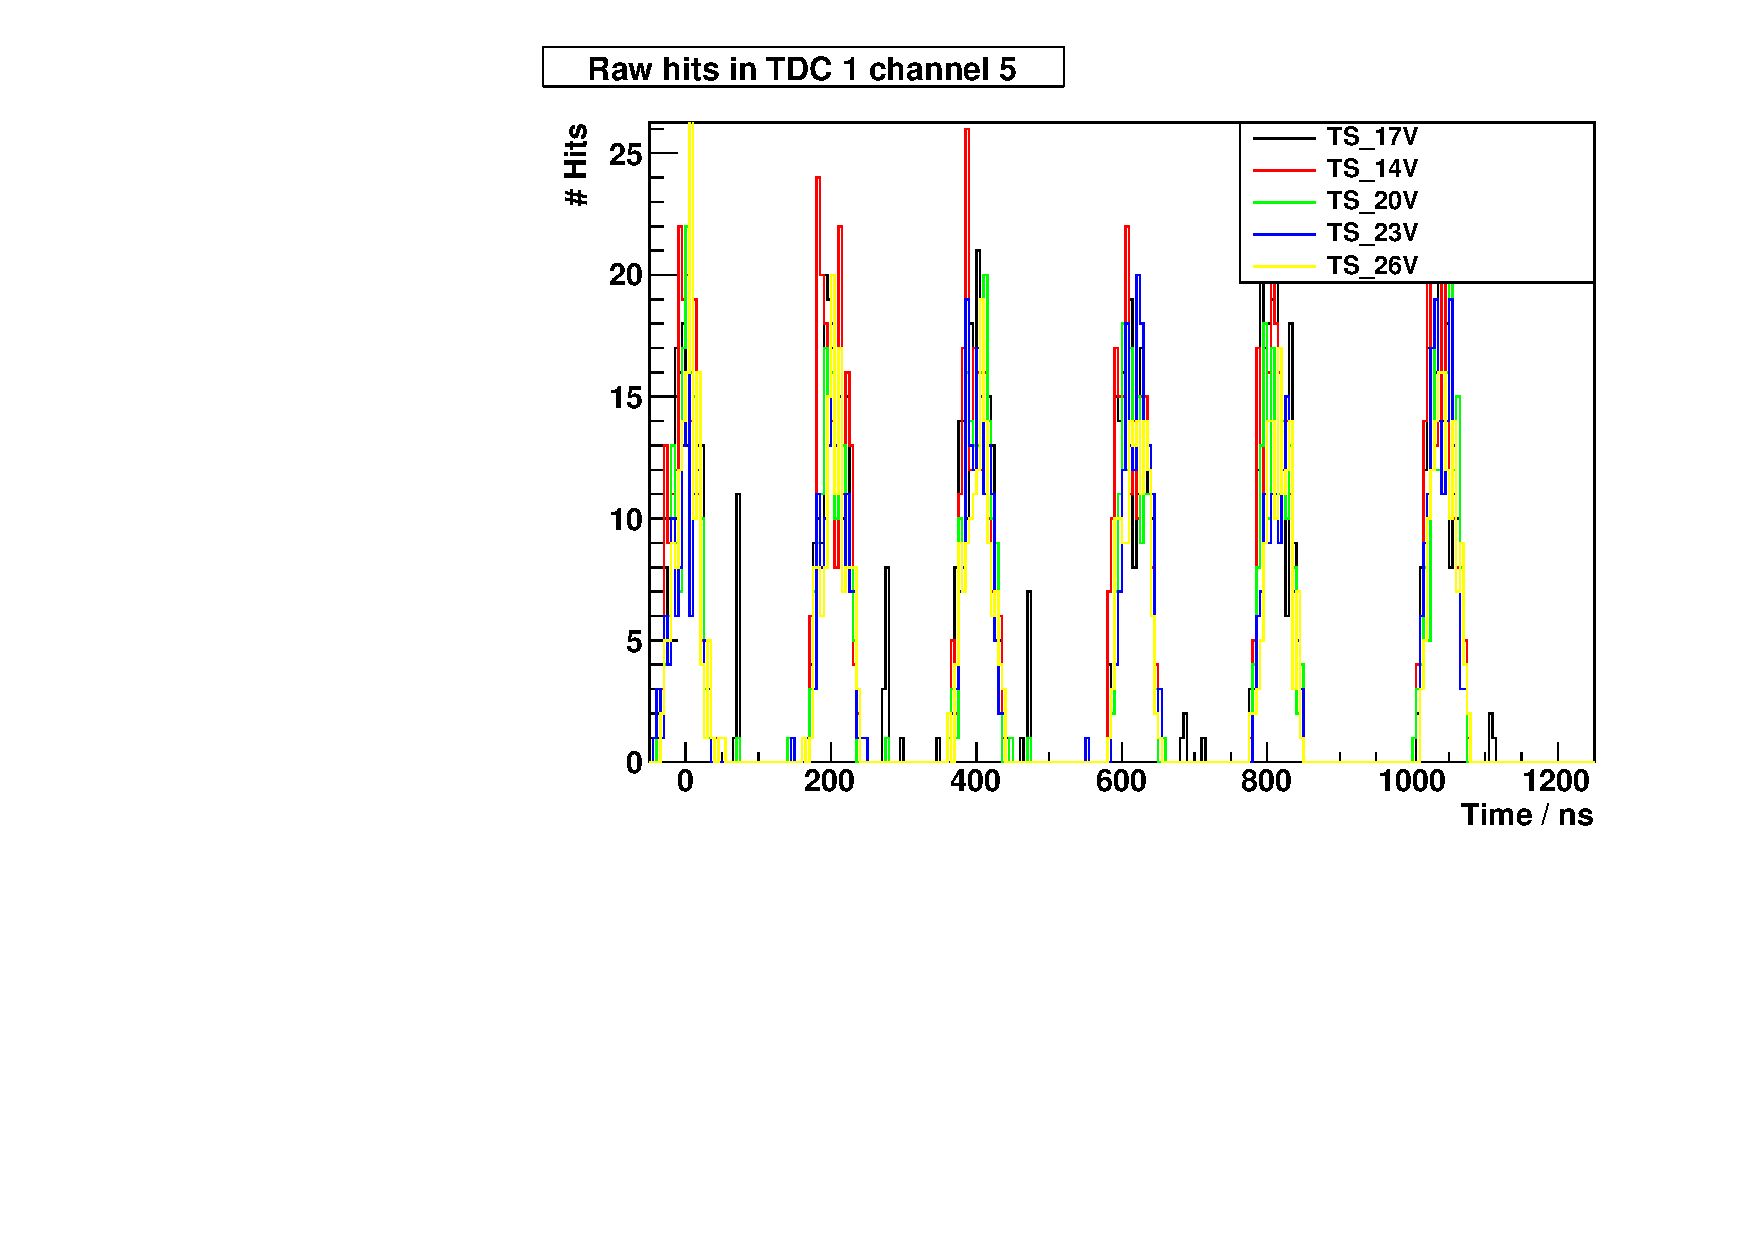
\includegraphics[width=0.8\linewidth]{StyxThresholdScan_1_5_Overlay.pdf}
 	\end{center}
 	\caption{In TDC 1 channel 5 at different voltages.}
 \end{subfigure}
 \caption{The overlay file of time-multiplexed vs hits}
 	\label{fig:Overlay}
 \end{figure}
 
 

 
	
